\documentclass[17pt, aspectratio=169]{beamer}

\usetheme{CambridgeUS}
\usecolortheme{dolphin}
\useinnertheme{rectangles}
\usepackage{svg}
\usepackage{setspace}
\usepackage{array}
\usepackage{multicol}
\usepackage[subpreambles=true]{standalone}
\usepackage{import}
\usepackage{xcolor}

\title{M.O.S.I.S Progress Report Presentation}
\author[Fabio J. \& Eduardo S.]{Fabio J. Matos Nieves \& Eduardo S. Miranda Figueroa}
\institute[UPRM]{University of Puerto Rico Mayagüez Campus}
\date{September 28, 2023}

\begin{document}
\begin{frame}
	\maketitle
\end{frame}
\begin{frame}{Table of Contents}
	\begin{multicols}{2}
		\begin{spacing}{0.8}
			\tableofcontents
		\end{spacing}
	\end{multicols}
\end{frame}
\section{Introduction}
\subsection{Problem Statement}
\begin{frame}{Problem Statement}
	\begin{itemize}
		\item The M.O.S.I.S microscope already has a user interface \textbf{but}:
		      \begin{itemize}
			      \item Lacks design cohesion
			      \item Missing and redundant features
			      \item Constantly crashes
			      \item Lacks a formal way to store data
		      \end{itemize}
	\end{itemize}
\end{frame}
\subsection*{Original Requirements}
\begin{frame}{Original Requirements}
	\begin{itemize}
		\item No camera control requirement
		\item Camera frame rate requirement was 15 frames per second
		\item No formal time stamp format 
	\end{itemize}
\end{frame}
\subsection*{Changes and Updates}
\begin{frame}{Changes and Updates}
	\begin{itemize}
		\item Client added camera control requirement to the project
		\item Client increased camera frame rate requirement to 24 frames per second
		\item Stakeholder clarified time stamp requirement (yyyy-MM-ddTHH:mm:ss.zzz)
	\end{itemize}
\end{frame}
\section{Body}
\subsection{Design Alternatives}
\begin{frame}{Design Alternatives}
	\begin{itemize}
		\item Browser Based
		\item Native
		\item Native Browser
	\end{itemize}
\end{frame}
\subsection*{Analysis Criteria}
\begin{frame}{Analysis Criteria}
	\begin{itemize}
		\item Minimized computing resource consumption
		      \begin{itemize}
			      \item CPU Cycles
			      \item System Memory Usage
			      \item Total System Power Draw
		      \end{itemize}
		\item Python Based
		\item Can easily be backed up and restored from a backup
	\end{itemize}
\end{frame}
\subsection*{Alternative Chosen}
\begin{frame}{Alternative Chosen}
	\begin{itemize}
		\item Native based app
		\item PyQt6 for U.I
		\item SQLite for Database
	\end{itemize}
\end{frame}
\subsection{System Architecture}
\subsubsection*{M.O.S.I.S UI 2.0}
\begin{frame}{M.O.S.I.S UI 2.0: System Architecture}
	\begin{figure}
		\resizebox{!}{0.65\textheight}{
			\import{../../Progress_Report_Document/Appendix/System_Architecture_and_Interfaces/Software_Architecture/Figures}{system_architecture}
		}
		\caption{System Architecture}
	\end{figure}
\end{frame}
\begin{frame}{M.O.S.I.S UI 2.0: Mock-ups (Preview)}
	\begin{figure}
		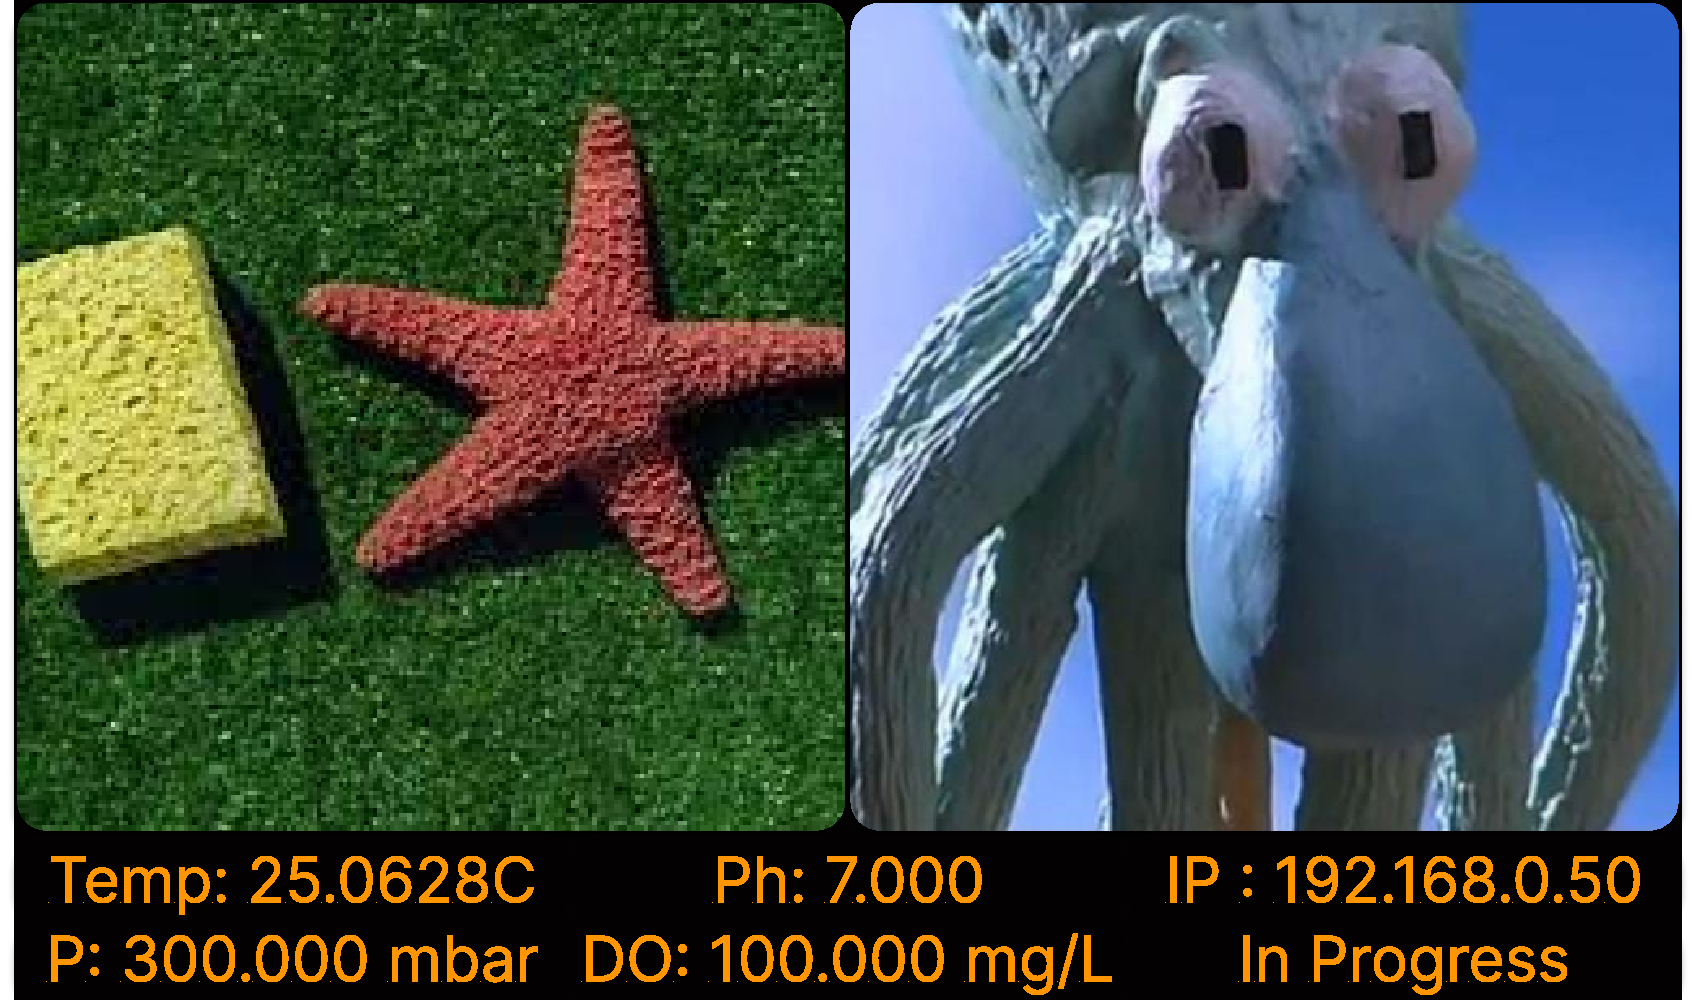
\includegraphics[page=1,height=0.65\textheight]{../../Progress_Report_Document/Appendix/Design_Documentation/User_Interface/Figures/M.O.S.I.S_UI_Design.pdf}
		\caption{Camera and Sensor Preview Mock-Up}
	\end{figure}
\end{frame}
\begin{frame}{M.O.S.I.S UI 2.0: Mock-ups (Study Select)}
	\begin{figure}
		\includegraphics[page=2,height=0.65\textheight]{../../Progress_Report_Document/Appendix/Design_Documentation/User_Interface/Figures/M.O.S.I.S_UI_Design.pdf}
		\caption{Study Select Menu Mock-Up}
	\end{figure}
\end{frame}
\begin{frame}{M.O.S.I.S UI 2.0: Mock-ups (Camera)}
	\begin{figure}
		\includegraphics[page=3,height=0.65\textheight]{../../Progress_Report_Document/Appendix/Design_Documentation/User_Interface/Figures/M.O.S.I.S_UI_Design.pdf}
		\caption{Camera Calibration Mock-Up}
	\end{figure}
\end{frame}
\begin{frame}{M.O.S.I.S UI 2.0: Mock-ups (Sensor)}
	\begin{figure}
		\includegraphics[page=7,height=0.65\textheight]{../../Progress_Report_Document/Appendix/Design_Documentation/User_Interface/Figures/M.O.S.I.S_UI_Design.pdf}
		\caption{Sensor Calibration Mock-Up}
	\end{figure}
\end{frame}
\begin{frame}{M.O.S.I.S UI 2.0: Class Diagram}
	\begin{figure}
		\resizebox{!}{0.65\textheight}{
			\import{../../Progress_Report_Document/Appendix/Design_Documentation/Class_Diagram/Figures/}{class_diagram}
		}
		\caption{Class Diagram}
	\end{figure}
\end{frame}
\begin{frame}{M.O.S.I.S UI 2.0: Entity Relationship Diagram}
	\begin{figure}
		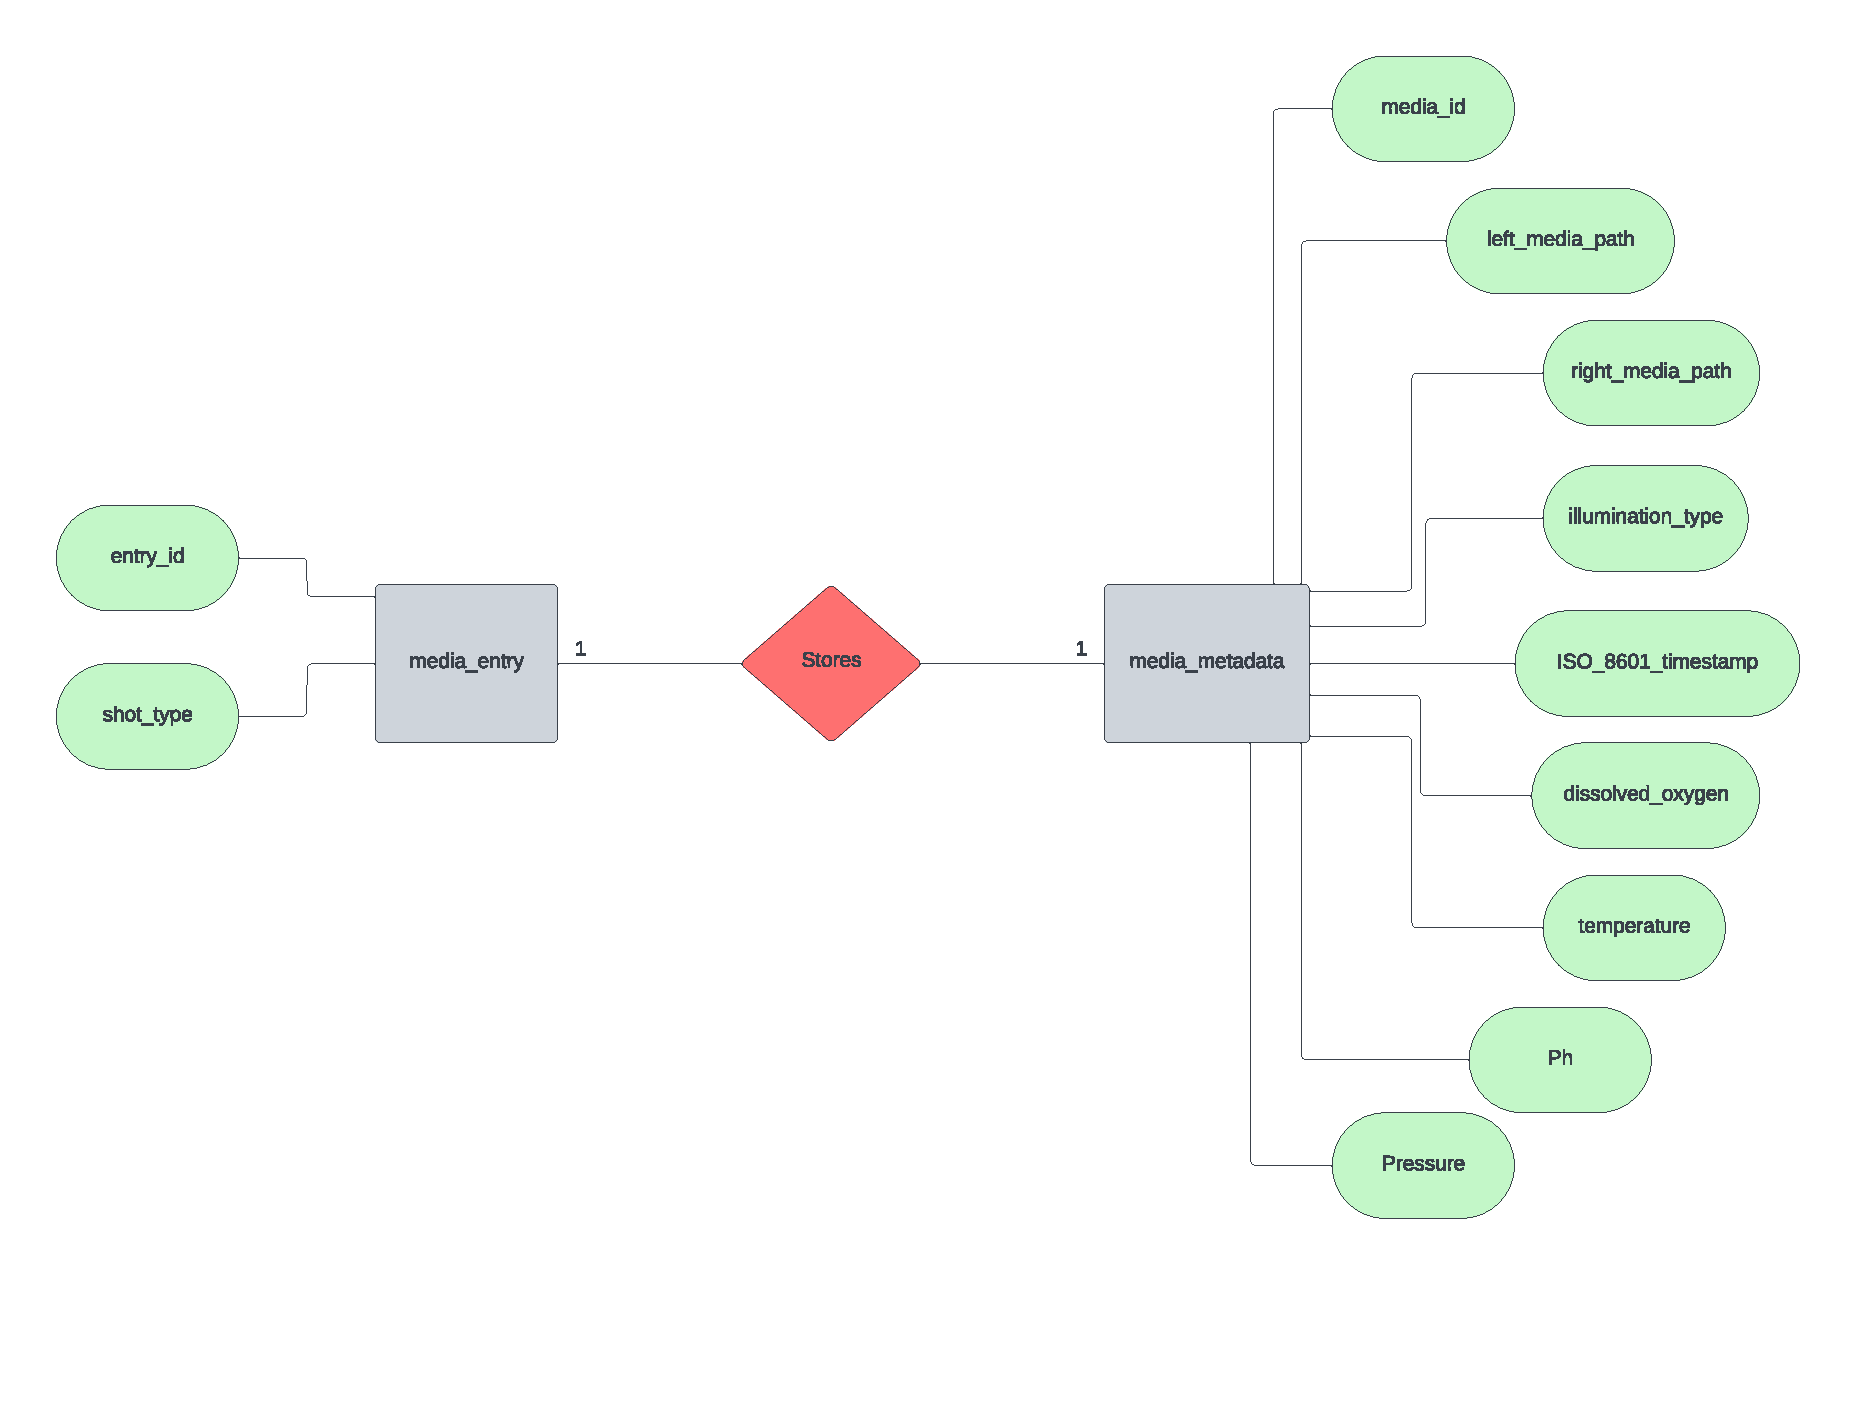
\includegraphics[page=1,height=0.65\textheight]{../../Progress_Report_Document/Appendix/Design_Documentation/ER_Diagram/Figures/ER_Diagram_MOSIS.pdf}
		\caption{ER Diagram}
	\end{figure}
\end{frame}
\subsubsection*{Firmware}
\begin{frame}{Cameras: Get Snapshot}
	\begin{figure}[H]
		\begin{center}
			\begin{small}
				\resizebox{!}{0.65\textheight}{
					\import{../../Progress_Report_Document/Appendix/Design_Documentation/Firmware_Flowcharts/Figures/}{get_snapshot_flowchart}
				}
			\end{small}
		\end{center}
		\caption{Get Snapshot Flowchart}
	\end{figure}
\end{frame}
\subsection{Project Status}
\begin{frame}{Project Status}
	\begin{itemize}
		\item M.O.S.I.S microscope unavailable from October 15 to October 21.
		      \begin{itemize}
			      \item Hardware API was originally going to be implemented from October 15 to October 30.
			      \item Now have to reassess the milestone timeline:
		      \end{itemize}
		      \begin{center}
			      \begin{tabular}{||c | c||}
				      \hline
				      Hardware API & Oct 15, 2023 \\
				      \hline
				      Back end API & Oct 15, 2023 \\
				      \hline
				      Front end    & Oct 30, 2023 \\
				      \hline
			      \end{tabular}
		      \end{center}
	\end{itemize}
\end{frame}
\subsection*{Deliverables}
\begin{frame}{Deliverables}
	\begin{center}
		\begin{tabular}{||c | c||}
			\hline
			Hardware API & Oct 15, 2023 \\
			\hline
			Back end API & Oct 15, 2023 \\
			\hline
			Front end    & Oct 30, 2023 \\
			\hline
		\end{tabular}
	\end{center}
	Before implementing the software we've finished the design mockups and schema for our back end API and front end.
\end{frame}
\subsection*{Current Budget}
\begin{frame}{Current Budget}
	\begin{center}
		\begin{tabular}{||m{0.75\textwidth} | m{0.20\textwidth} ||}
			\hline
			Eduardo S. Miranda \& Fabio J. Matos's Salary& \$6,270.00\\
			\hline
			Facility Cost & \$470.00 \\
			\hline
			Udemy "Python GUI Development with PyQt6 \& Qt Designer" Class & \$28.98 \\
			\hline
			Total Current Budget Cost & \$9,562.4\\
			\hline
		\end{tabular}
\end{center}
\end{frame}
\section{Conclusion}
\subsection{Accomplishments}
\begin{frame}{Accomplishments}
	\begin{itemize}
		\item Finished the Udemy course on PyQt6
		\item Worked on U.I mock ups
		\item Worked on Design Schema for Database
	\end{itemize}
\end{frame}
\subsection*{Expenditure and Budget Status}
\begin{frame}{Expenditure and Budget Status}
\begin{itemize}
	\item Estimated Budget Cost = \$41,703.03 
	\item Actual Budget Cost = \$29,804.22 
	\item Difference in Budget Cost = \textcolor{teal}{-\$11,900.81}
\end{itemize}
\end{frame}
\subsection{Future Work}
\begin{frame}{Future Work}
We will start on the hardware API and backend API as soon as the mock ups are approved, before October 15. After finishing those milestones we will begin on the front end.
\end{frame}
\subsection*{Questions}
\begin{frame}
	\begin{huge}
	\begin{center}
		Questions?
	\end{center} 
\end{huge}
	\end{frame}
\end{document}